\section{Natalia Kuchta}

\begin{figure}[h]
    \centering
    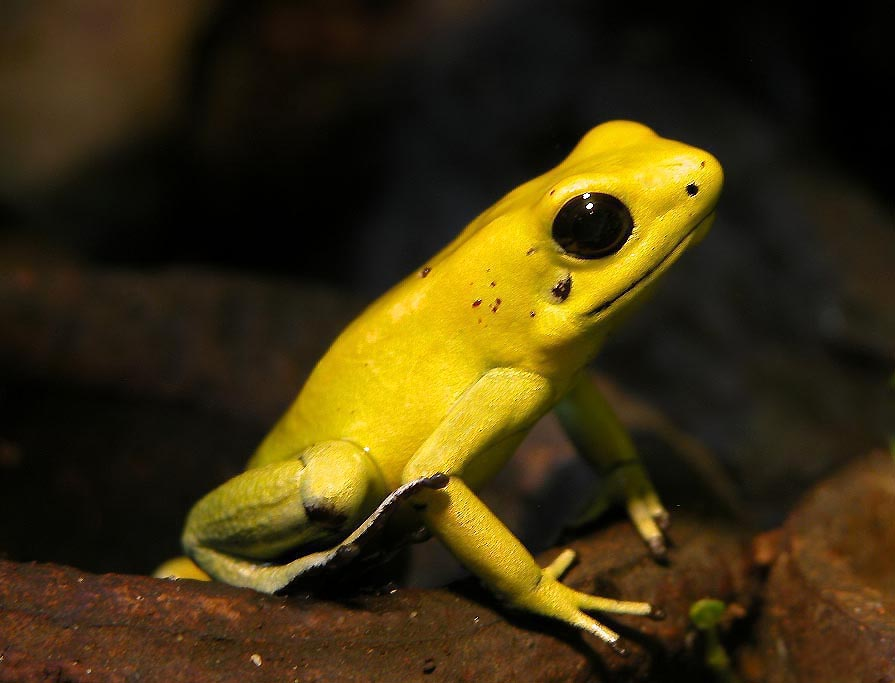
\includegraphics{pictures/zaba.jpg}
    \caption{Golden poison frog}
    \label{fig:frog}
\end{figure}
\begin{flushleft}
    \textbf{Golden poison frog} (alternative names: \textit{golden dart frog, golden poison arrow frog}) is one of the most \underline{poisonous} animals that live on Earth. They skin secretions contain deadly alkaloid. Their poison level is so high even touching them can result in tragic consequences. They are quite crucial for local indigenous cultures, as they provide the main source of poison which is used in the darts used by natives while hunting. 

They can be found in rain forests of Colombia. They weight nearly 30 grams and are about 6 cm long. Before reaching adulthood, golden poison frogs have mostly black bodies with two yellow stripes visible on their backs.    
\end{flushleft}
They occur in four color varieties:
\begin{itemize}
    \item Yellow
    \item Mint green
    \item Orange
    \item Orange blackfoot
\end{itemize}

In the picture ~\ref{fig:frog} you can see a golden poison frog.

List number 2
\begin{enumerate}
    \item One
    \item Two
    \item Three
\end{enumerate}

\begin{center}
\begin{table}[]
\begin{tabular}{| c | c | c | c |}
\hline
\textbf{alpha} & \textbf{0} & \textbf{90} & \textbf{180} \\
\hline
\textbf{sin}   & 0          & 1           & 0            \\
\hline
\textbf{cos}   & 1          & 0           & -1           \\
\hline
\textbf{tg}    & 0          & -           & 0          \\
\hline
\end{tabular}
\label{tab:sincostg}
\end{table}


Table~\ref{tab:sincostg} represents some values of trigonometric functions.
\end{center}

\[sin^2\alpha + cos^2\alpha = 1\]




